% !TEX TS-program = pdflatex
% !TEX encoding = UTF-8 Unicode

% This is a simple template for a LaTeX document using the "article" class.
% See "book", "report", "letter" for other types of document.

\documentclass[11pt]{article} % use larger type; default would be 10pt

\usepackage[utf8]{inputenc} % set input encoding (not needed with XeLaTeX)

%%% Examples of Article customizations
% These packages are optional, depending whether you want the features they provide.
% See the LaTeX Companion or other references for full information.

%%% PAGE DIMENSIONS
\usepackage{geometry} % to change the page dimensions
\geometry{a4paper} % or letterpaper (US) or a5paper or....
% \geometry{margins=2in} % for example, change the margins to 2 inches all round
% \geometry{landscape} % set up the page for landscape
%   read geometry.pdf for detailed page layout information

\usepackage{graphicx} % support the \includegraphics command and options

% \usepackage[parfill]{parskip} % Activate to begin paragraphs with an empty line rather than an indent

%%% PACKAGES
\usepackage{booktabs} % for much better looking tables
\usepackage{array} % for better arrays (eg matrices) in maths
\usepackage{paralist} % very flexible & customisable lists (eg. enumerate/itemize, etc.)
\usepackage{verbatim} % adds environment for commenting out blocks of text & for better verbatim
\usepackage{subfig} % make it possible to include more than one captioned figure/table in a single float
% These packages are all incorporated in the memoir class to one degree or another...

\usepackage{graphicx}
\usepackage{float}

\usepackage{tabularx}


\usepackage{color}
\usepackage{xcolor}
\usepackage{listings}
\usepackage{caption}
\DeclareCaptionFont{white}{\color{white}}
\DeclareCaptionFormat{listing}{\colorbox{gray}{\parbox{\textwidth}{#1#2#3}}}
\captionsetup[lstlisting]{format=listing,labelfont=white,textfont=white}


%%% HEADERS & FOOTERS
\usepackage{fancyhdr} % This should be set AFTER setting up the page geometry
\pagestyle{fancy} % options: empty , plain , fancy
\renewcommand{\headrulewidth}{0pt} % customise the layout...
\lhead{}\chead{}\rhead{}
\lfoot{}\cfoot{\thepage}\rfoot{}

%%% SECTION TITLE APPEARANCE
\usepackage{sectsty}
\allsectionsfont{\sffamily\mdseries\upshape} % (See the fntguide.pdf for font help)
% (This matches ConTeXt defaults)

%%% ToC (table of contents) APPEARANCE
\usepackage[nottoc,notlof,notlot]{tocbibind} % Put the bibliography in the ToC
\usepackage[titles,subfigure]{tocloft} % Alter the style of the Table of Contents
\renewcommand{\cftsecfont}{\rmfamily\mdseries\upshape}
\renewcommand{\cftsecpagefont}{\rmfamily\mdseries\upshape} % No bold!

%%% END Article customizations

%%% The "real" document content comes below...

\title{Brief Article}
\author{The Author}
%\date{} % Activate to display a given date or no date (if empty),
         % otherwise the current date is printed 

\begin{document}
\maketitle


\section{Task Knowledge}


\section{Inference Knowledge}

As inference model we use a modified version of the Configuration design template, because given predefined components we need to find and assembly that satisfies the requirements. The inference model deriving from this task can be found in Figure~\ref{fig:inference}.

\begin{figure}[h]
\centering
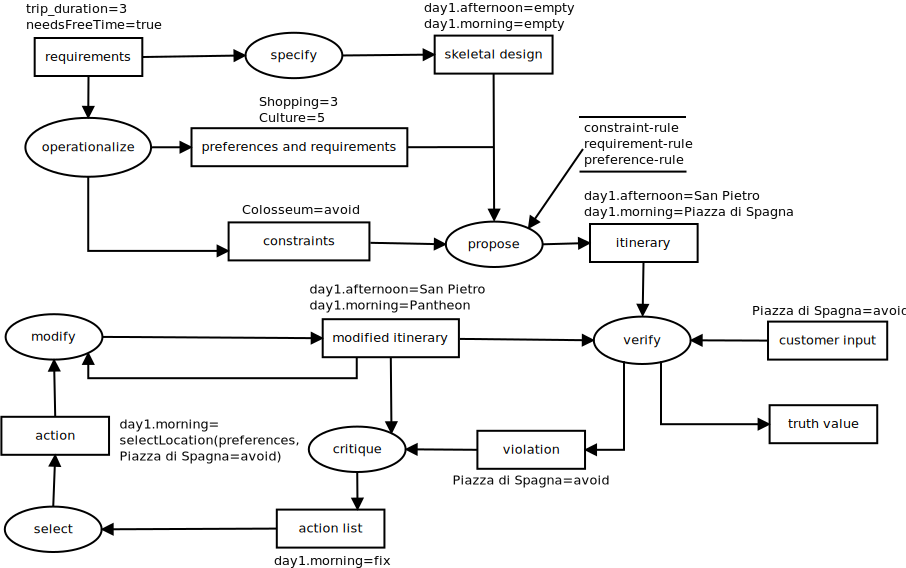
\includegraphics[width=\textwidth]{images/inference.pdf}
\caption{Inference structure}
\label{fig:inference}
\end{figure}

\noindent
\begin{tabularx}{\textwidth}{| X | X | X | X |}
  \hline
inference		& Input	& Output 	& Description \\ \hline \hline
specify		& requirements	& sketal design		& the function look-up the default sketal design: the basic structure of a trip day (heavy activity during the morning, relaxing afternoon, evening and meal).
\\ \hline 
   optionalize	& needs of the customers		& preferences, requirements, constraints	& the needs and desires are translated into preferences ("I would like to have time for shopping and visit many cultural places. I am not interested so much in food places"), requirements ("I want a quiet trip") and contraints ("In Rome I want to visit the \emph{Colosseum} and avoid \emph{Piazza di Spagna}"). 
\\ \hline
propose	& preferences and requirements, sketal design slots		& filled sketal design	& fill the slots of the sketal design with locations that fits the preferences and requirements.
\\ \hline
\end{tabularx}
\noindent
\begin{tabularx}{\textwidth}{| X | X | X | X |}
\hline
verify		& contraints, extension design	& the list of violated contraints	& it checks with the help of the internal contraints and those supplied by the user whether the current configuration is internally consistent. If the verification fails, it produces the violated contraints as an additional output
\\ \hline
select 	& fix actions list		& fix action		& It simply selects an action from the fix actions list generated by the critique function.
\\ \hline
modify	& itinerary design, fix actions list		& fixed itinerary design		& it applies the fix actions to the design.
\\ \hline
critique	& itinerary, violations, customer's inputs	& fix actions list		& it creates a series of actions which will fix the violations of the contraints, following also the customer's inputs. For example the contraint "I absolutely want to visit the \emph{Colosseum}" will produce the action "Insert the \emph{Colosseum} into the itinerary".
\\ \hline
\end{tabularx}

%TOBEDONE: forse dobbiamo commentare i knwoledge roles?


\section{Domain knowledge}

%TOBEDONE: spiegare un po' le sorgenti di questo schema? Tipo risultati dell'intervista ecc? ma forse dobbiamo dirlo ben prima

\subsection{Domain schema}
The domain schema can be found in Figure~\ref{fig:ClassDiagram}

\begin{figure}[h]
\centering
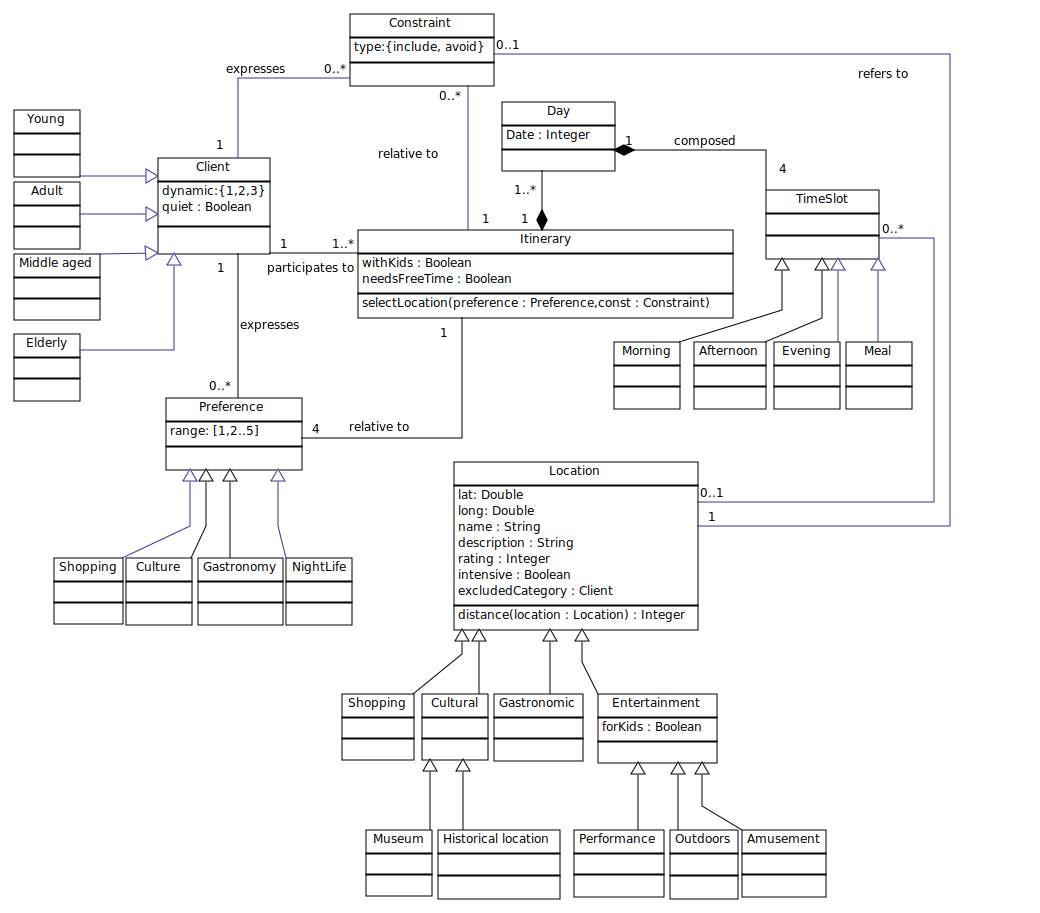
\includegraphics[width=\textwidth]{images/ClassDiagram.pdf}
\caption{Domain schema}
\label{fig:ClassDiagram}
\end{figure}


This schema seems complicated, for this reason every model is explained in the following list:
\begin{description}
  \item[Client] \hfill \\
  The client who goes to the travel agency. He could be a quite person who normally wants to visit a lot of things or very few (\emph{dynamic}). The clients are categorized by their age because some locations are not suitable for a people category (ex: elderly people in a climbing location).

  \item[Preference] \hfill \\
  Each client needs to specify a list of preferences, valued from 1 to 5, where 1 is "I'm not so interested" and 5 is "I love to do it!". These preferences are related to the itinerary we want to create, consequently if the same clients wants to create another itinerary, it will specify again all the preferences he wants in this second trip.
  \item[Contraint] \hfill \\
  Each client needs to specify a list of contraints that have to be fulfilled. As for the \emph{Preference}, they are related to the single itinerary.
  \item[Itinerary] \hfill \\
  This represents the itinerary we want to create. It is composed by a fixed number of \emph{Day} and it is related to a \emph{Client} who has specified his own list of \emph{Contraint} and \emph{Preference}. If there will be kids in the itinerary, the system needs to select some \emph{Location} that could entertain them. This is a requirement as the \emph{needsFreeTime} attribute, which specifies that the clients needs to have some not scheduled time in the arrival city.\\
The method \emph{selectLocation} takes a list of \emph{Preference} and produces a list of \emph{Location} that could fit this preferences. 
  \item[Day] \hfill \\
  This describes a day of the itinerary.
  \item[Timeslot] \hfill \\
  A timeslot is a fixed part of a day. The division of the day came from the expert interview.
\item[Location] \hfill \\
  This model represents the point of interests that a customer could visit. The attribute \emph{rating} describes the quality of this place, \emph{intensive} describes if the place is not for quite people and \emph{excludedCategory} specifies if a client category is not suitable for the location (ex: elderly people in a climbing location). The method \emph{distance} takes two locations and returns the distance between them. It is useful in order to create the combination of locations to visit during a trip.
\end{description}

%TOBEDONE: Domain schema with rule types

\subsection{Rule types}

\begin{lstlisting}[label=Rules,caption=Rules,breaklines=true]
RULE TYPE constraint-rule;
    DESCRIPTION: "rule stating the relation between client and the choice for a location in the itinerary, by means of defining strict boundaries that must be respected.";
ANTECEDENT: Client;
CONSEQUENT: Itinerary;
CONNECTION-SYMBOL: restricts;
END RULE-TYPE constraint-rule;

RULE TYPE requirement-rule;
    DESCRIPTION: "rule stating the relation between the client and the choice for a location in the itinerary, by means of defining boundaries that should be respected.";
ANTECEDENT: Client;
CONSEQUENT: Itinerary;
CONNECTION-SYMBOL: requires;
END RULE-TYPE requirement-rule;

RULE TYPE preference-rule;
    DESCRIPTION: "rule stating the relation between the client and the choice for a location in the itinerary, by means of defining preferences that could be satisfied with probability X (calculated on the input values) .";
ANTECEDENT: Client;
CONSEQUENT: Itinerary;
CONNECTION-SYMBOL: prefers-with-probability;
END RULE-TYPE preference-rule;
\end{lstlisting}


\noindent
Here are presented also some example in order to better understand all the rule types.

\begin{lstlisting}[label=Rules,caption=The client wants to include a destination into the itinerary.,breaklines=true,mathescape=true]
client.constraint.location.name$=$A AND client.constraint.type$=$include
RESTRICTS
$\exists$itinerary.day.timeslot, timeslot.location.name$=$A;
\end{lstlisting}



%TOBEDONE!!!!
\begin{lstlisting}[label=Rules,caption=The client is a quite person,breaklines=true,mathescape=true]
client.quiet=true, client.needsFreeTime=true, client.active=1
REQUIRES
itinerary.day.timeslot.location, location.intensive=false;
itinerary.day.timeslot, timeslot.location=NULL;
$\sum_{i=1}^{n-1}$i.distance(i+1) $<\delta$, $\forall$i $\in$ location;
\end{lstlisting}




\begin{lstlisting}[label=Rules,caption=The client expresses four preferences with four ranges (from 1 to 5). The method selectLocation will compose the itinerary selecting the locations that fits the preferences. For example it could select 3 shopping\, 1 gastronomy and 1 cultural locations.,breaklines=true,mathescape=true]
Var A, B, C, D: client.preference;
Var E: client.constraint;
A.type=shopping AND A.range=x
B.type=cultural AND B.range=y
C.type=gastronomy AND C.range=w
D.type=nightlife AND D.range=z
E.type = avoid AND E.location = Colusseum
PREFERS-WITH-PROBABILITY
$\forall$itinerary.day.timeslot, timeslot.location=selectLocation(A, B, C, D, E);
\end{lstlisting}

\subsection{Knowledge Base}

\begin{figure}[h]
\centering
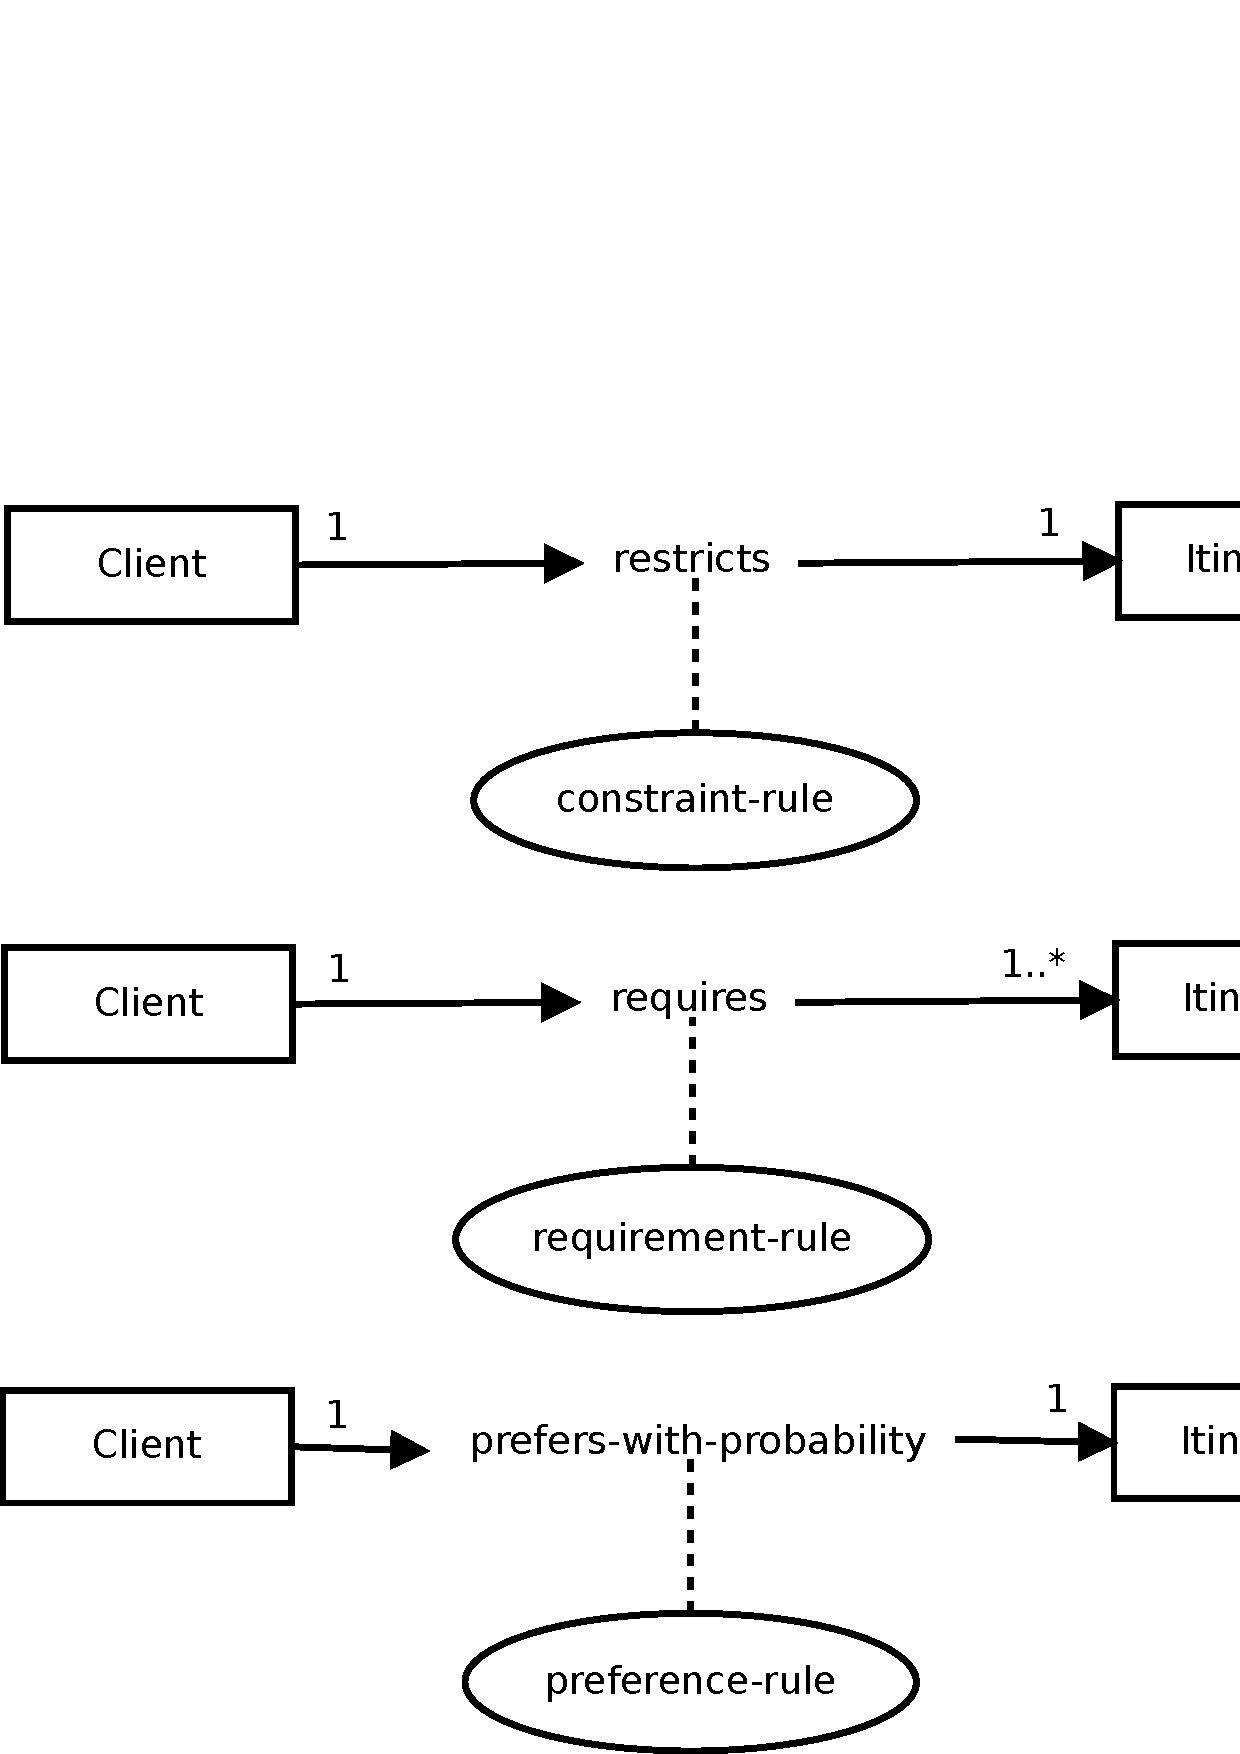
\includegraphics[height=7cm]{images/knowledge_base.pdf}
\caption{Knowledge base}
\label{fig:knowledgebase}
\end{figure}



\section{Scenarios}



\end{document}
